\documentclass[12pt]{report}
\usepackage[utf8]{inputenc}
\usepackage[russian]{babel}
%\usepackage[14pt]{extsizes}
\usepackage{listings}
\usepackage{pdfpages}

% Для листинга кода:
\lstset{ %
language=python,                 % выбор языка для подсветки (здесь это С)
basicstyle=\small\sffamily, % размер и начертание шрифта для подсветки кода
numbers=left,               % где поставить нумерацию строк (слева\справа)
numberstyle=\tiny,           % размер шрифта для номеров строк
stepnumber=1,                   % размер шага между двумя номерами строк
numbersep=5pt,                % как далеко отстоят номера строк от подсвечиваемого кода
showspaces=false,            % показывать или нет пробелы специальными отступами
showstringspaces=false,      % показывать или нет пробелы в строках
showtabs=false,             % показывать или нет табуляцию в строках            
tabsize=2,                 % размер табуляции по умолчанию равен 2 пробелам
captionpos=t,              % позиция заголовка вверху [t] или внизу [b] 
breaklines=true,           % автоматически переносить строки (да\нет)
breakatwhitespace=false, % переносить строки только если есть пробел
escapeinside={\#*}{*)}   % если нужно добавить комментарии в коде
}

% Для измененных титулов глав:
\usepackage{titlesec, blindtext, color} % подключаем нужные пакеты
\definecolor{gray75}{gray}{0.75} % определяем цвет
\newcommand{\hsp}{\hspace{20pt}} % длина линии в 20pt
% titleformat определяет стиль
\titleformat{\chapter}[hang]{\Huge\bfseries}{\thechapter\hsp\textcolor{gray75}{|}\hsp}{0pt}{\Huge\bfseries}


% plot
\usepackage{pgfplots}
\usepackage{filecontents}
\usetikzlibrary{datavisualization}
\usetikzlibrary{datavisualization.formats.functions}
\begin{filecontents}{BubbleNotSorted.dat}
100 880860
200 2889780
300 6841660
400 12311020
500 19054280
600 27940100
700 40081620
800 52825900
900 68077780
1000 83859160
\end{filecontents}
\begin{filecontents}{BubbleSortedUp.dat}
100 516880
200 1653920
300 3772320
400 7113740
500 11206320
600 16688120
700 23531260
800 30523940
900 40099680
1000 50063820
\end{filecontents}
\begin{filecontents}{BubbleSortedDown.dat}
100 1247240
200 4258960
300 9609200
400 17442180
500 27016920
600 39748560
700 54505880
800 71409520
900 92583200
1000 116075660
\end{filecontents}

\begin{filecontents}{InsertNotSorted.dat}
100 507360
200 1657440
300 3952480
400 7125920
500 10794400
600 16160200
700 24159040
800 32081600
900 41336920
1000 51096940
\end{filecontents}
\begin{filecontents}{InsertSortedUp.dat}
100 22920
200 38820
300 52400
400 73340
500 96280
600 118780
700 142420
800 168100
900 189960
1000 222380
\end{filecontents}
\begin{filecontents}{InsertSortedDown.dat}
100 982080
200 3416020
300 7488760
400 13676340
500 22467280
600 33145800
700 46267700
800 63021940
900 81096820
1000 101704340
\end{filecontents}

\begin{filecontents}{QuickNotSorted.dat}
100 640540
200 1243740
300 1737740
400 2406620
500 3157300
600 3982980
700 4684940
800 5526180
900 6351480
1000 7488500
\end{filecontents}
\begin{filecontents}{QuickSortedUp.dat}
100 582880
200 1072540
300 1702240
400 2387660
500 3117760
600 3848740
700 4649540
800 5393340
900 6144640
1000 7291560
\end{filecontents}
\begin{filecontents}{QuickSortedDown.dat}
100 596520
200 1221800
300 1706220
400 2456200
500 3042160
600 3850960
700 4680000
800 5410000
900 6105680
1000 7191500
\end{filecontents}

\usepackage{graphicx}
\graphicspath{{src/}}
\DeclareGraphicsExtensions{.pdf,.png,.jpg}

\begin{document}
%\def\chaptername{} % убирает "Глава"

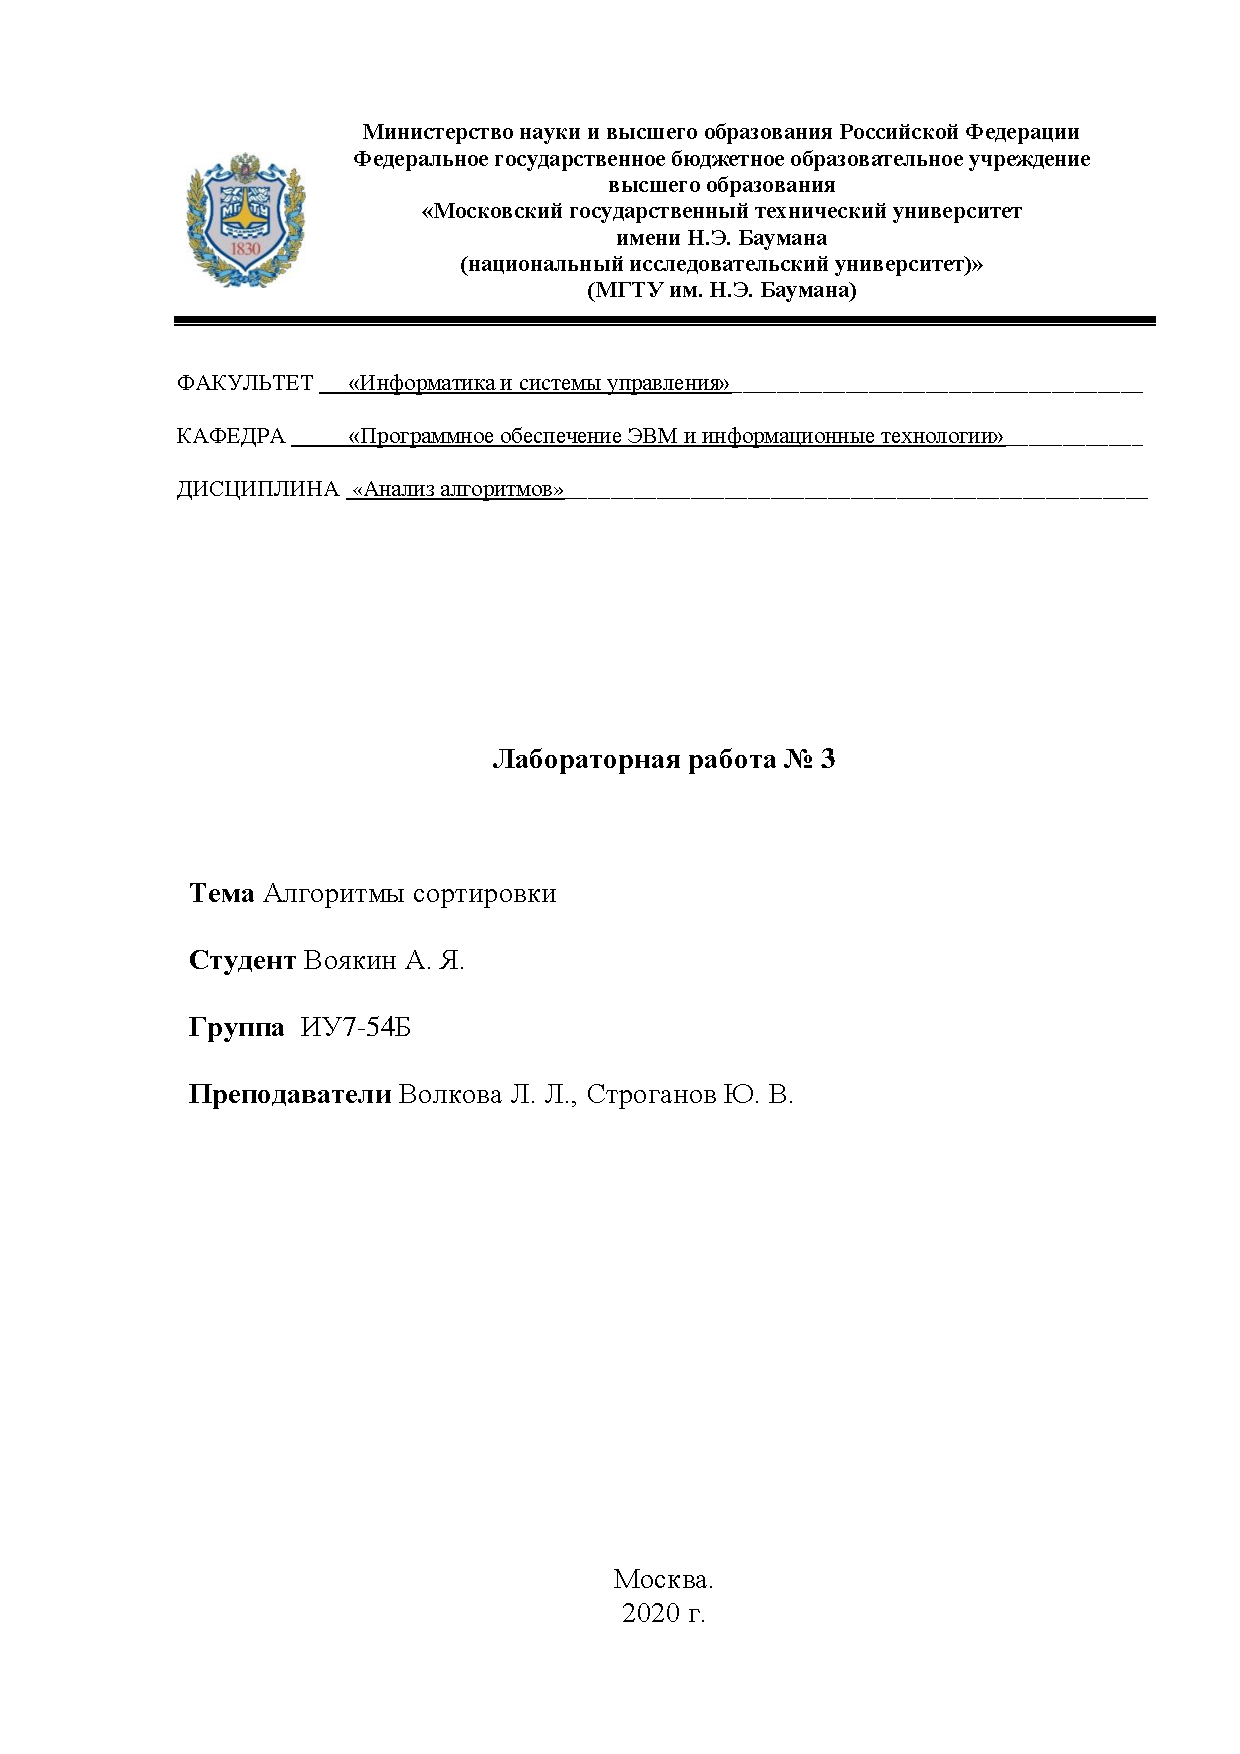
\includepdf{Title.pdf}

\tableofcontents

\newpage
\chapter*{Введение}
\addcontentsline{toc}{chapter}{Введение}

На сегодняшний день существует не одна вариация алгоритмов сортировки. Все они различаются по скорости сортировки и по объему необходимой памяти. 

Цель данной лабораторной работы - обучение расчету трудоемкости алгоритмов

Алгоритмы сортировки часто применяются в практике программирования. В том числе в областях связанных с математикой, физикой, компьютерной графикой и т.д.

В ходе лабораторной работы предстоит:
\begin{itemize}
	\item изучить алгоритмы сортировок;
	\item дать теоретическую оценку алгоритмам сортировки;
	\item реализовать три алгоритма сортировки на одном из языков программирования;  
	\item сравнить алгоритмы сортировок.
\end{itemize}

\chapter{Аналитическая часть}
\section{Сортировка пузырьком}
Алгоритм состоит из повторяющихся проходов по сортируемому массиву. За каждый проход элементы последовательно сравниваются попарно и, если порядок в паре неверный, выполняется обмен элементов.

\section{Сортировка вставками}
На каждом шаге выбирается один из элементов неотсортированной части массива (максимальный/минимальный) 
и помещается на нужную позицию в отсортированную часть массива. 

\section{Быстрая сортировка}
Общая идея алгоритма состоит в следующем:

\begin{enumerate}
  	\item Выбрать из массива элемент, называемый опорным. Это может быть любой из элементов массива. От выбора опорного элемента не зависит корректность алгоритма, но в отдельных случаях может сильно зависеть его эффективность.
	\item Сравнить все остальные элементы с опорным и переставить их в массиве так, чтобы разбить массив на три непрерывных отрезка, следующих друг за другом: «элементы меньшие опорного», «равные» и «большие».
	\item Для отрезков «меньших» и «больших» значений выполнить рекурсивно ту же последовательность операций, если длина отрезка больше единицы.
\end{enumerate}
На практике массив обычно делят не на три, а на две части: например, «меньшие опорного» и «равные и большие»; такой подход в общем случае эффективнее, так как упрощает алгоритм разделения

\section{Вывод}
В данном разделе были рассмотрены три алгоритма сортироки.

\chapter{Конструкторская часть}
\section{Схемы алгоритмов}

На рисунке (\ref{ris:imageBubble}) приведена схема классического алгоритма сортировки пузырьком.\\
На рисунке (\ref{ris:imageInsert}) приведена схема алгоритма сортировки вставками.\\
На рисунке (\ref{ris:imageQuick}) приведена схема быстрой сортировки.

\begin{figure}
	\begin{center}
	{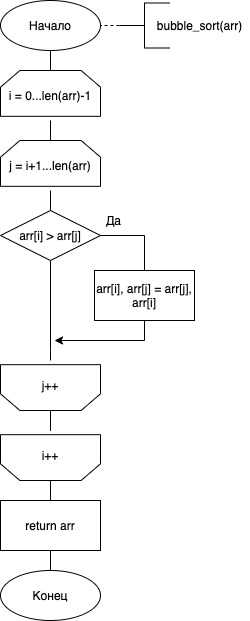
\includegraphics[height = 18cm]{bubble.jpg}}
	\caption{Схема алгоритма сортировки пузырьком}
	\label{ris:imageBubble}
	\end{center}
\end{figure}
	
\begin{figure}
	\begin{center}
	{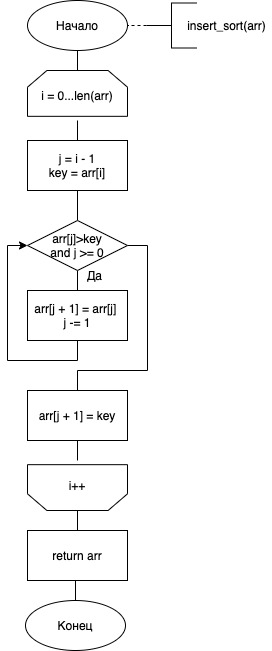
\includegraphics[height = 18cm]{insert.jpg}}
	\caption{Схема алгоритма сортировки вставками}
	\label{ris:imageInsert}
	\end{center}
\end{figure}

\begin{figure}
	\begin{center}
	{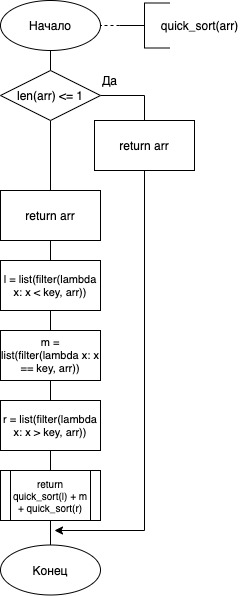
\includegraphics[height = 18cm]{quick.jpg}}
	\caption{Схема алгоритма быстрой сортировки}
	\label{ris:imageQuick}
	\end{center}
\end{figure}


\newpage
\section{Трудоемкость алгоритмов}
Введем модель трудоемкости для оценки алгоритмов:
\begin{enumerate}
  	\item  базовые операции стоимостью 1 — +, -, *, /, =, ==, <=, >=, !=, +=, [], ++, -- получение полей класса
	\item оценка трудоемкости цикла: Fц = a + N*(a + Fтела), где a - условие цикла
	\item стоимость условного перехода возьмем за 0, стоимость вычисления условия остаётся.
\end{enumerate}

Далее будет приведены оценки трудоемкости алгоритмов. Построчная оценка трудоемкости сортировки пузырькм с флагом (Табл. 2.1).

\subsection{Сортировка пузырьком}
\textbf{Лучший случай:} Массив отсортирован; не произошло ни одного обмена за 1 проход -> выходим из цикла \newline
Трудоемкость:  $1+2n*(1 + 2n*4) = 1+2n+16n*n=  O(n^{2})$

\textbf{Худший случай:}  Массив отсортирован в обратном порядке; в каждом случае происходил обмен\newline
Трудоемкость: $1+2n*(1 + 2n*(4+5)) = O(n^2)$

\subsection{Сортировка вставками}
\begin{center}
Табл. 2.1 Построчная оценка веса
	\begin{tabular}{|l c|} 
 	\hline
	Код & Вес \\ [0.5ex] 
 	\hline
 	for i in range(1, len(a)): & 1+n*2\\
 	\hline
	key = a[i] & 2\\
	\hline
	j = i-1 & 2\\
	\hline
	while (j >= 0 and a[j] > key): & n*4\\
	\hline
	a[j+1] = a[j] & 4\\
	\hline
	\j -= 1 & 1\\
	\hline
	a[j+1] = key & 3\\
	\hline
	\end{tabular}
\end{center}

\hspace*{5mm}
\textbf{Лучший случай:} отсортированный массив. При этом все внутренние циклы состоят всего из одной итерации.\newline
Трудоемкость: $T(n) = 1 + 2n * (2+2+3)  =  2n * 7 = 14n + 1 = O(n)$

\textbf{Худший случай:} массив отсортирован в обратном нужному порядке. Каждый новый элемент сравнивается со всеми в отсортированной последовательности.
Все внутренние циклы будут состоять из j итераций. \newline
Трудоемкость: $T(n) = 1+n*(2+2+4n*(4+1)+3) = 2n*n+7n+1 =  O(n^{2})$


\subsection{Быстрая сортировка}
\hspace*{5mm}
\textbf{Лучший случай:} сбалансированное дерево вызовов$^{[2]}$ \(O(n*log(n))\)  
В наиболее благоприятном случае процедура PARTITION приводит к двум подзадачам, размер каждой из которых не превышает $\frac{n}{2}$, поскольку размер одной из них равен $\frac{n}{2}$ , а второй$\frac{n}{2} - 1$. В такой ситуации быстрая сортировка работает намного производительнее, и время ее работы описывается следующим рекуррентным соотношением: $T(n) = 2T(\frac{n}{2}) + O(n)$,где мы не обращаем внимания на неточность, связанную с игнорированием функций “пол” и “потолок”, и вычитанием 1. Это рекуррентное соотношение имеет решение ; $T(n) =O(nlgn)$. При сбалансированности двух частей разбиения на каждом уровне рекурсии мы получаем асимптотически более быстрый алгоритм.

Фактически любое разбиение, характеризующееся конечной константой пропорциональности, приводит к образованию дерева рекурсии высотой $O(lgn)$ со стоимостью каждого уровня, равной $O(n)$. Следовательно, прилюбой постоянной пропорции разбиения полное время работы быстрой сортировки составляет $O(nlgn)$.

\textbf{Худший случай:} несбалансированное дерево $^{[2]}$ $O(n^2)$
Поскольку рекурсивный вызов процедуры разбиения, на вход которой подается массив размером 0, приводит к немедленному возврату из этой процедуры без выполнения каких-ли-бо операций, $T(0) = O(1)$. Таким образом, рекуррентное соотношение, описывающее время работы процедуры в указанном случае, записывается следующим образом: 
$T(n) =T(n-1) +T(0) + O(n) =T(n-1) + O(n)$. Интуитивно понятно, что при суммировании промежутков времени, затрачиваемых на каждый уровень рекурсии, получается арифметическая прогрессия, что приводит к результату $O(n^2)$.

\section{Вывод}
Сортировка пузырьком: лучший - $O(n)$, худший - $O(n^2)$ \newline
Сортировка вставками: лучший - $O(n)$, худший - $O(n^2)$ \newline
Быстрая сортировка: лучший - $O(nlgn)$, худший - $O(n^2)$ \newline

\chapter{Технологическая часть}
\section{Выбор ЯП}
Был  выбран Python в качестве языка программирования, потому как он достаточно удобен и гибок. Среда разработки PyCharm.

Время работы алгоритмов было замерено с помощью функции process\_time\_ns() из библиотеки time.

\section{Сведения о модулях программы}
Программа состоит из:
\begin{itemize}
	\item lab03.py - файл, в котором находятся функции сортировки
	\item time\_test.py - файл, в котором реализовано тестировние алгоритмов по времени
\end{itemize}

\section{Листинг кода}

В листингах 3.1 - 3.3 приведены реализации алгоритмов сортировки массивов.\\
В листинге  3.4 приведена реализация функции замера процессорного времени.

\begin{lstlisting}[label=some-code,caption=Сортировка пузырьком]
def bubble_sort(arr):
	for i in range(len(arr) - 1):
		for j in range(i + 1, len(arr)):
			if arr[i] > arr[j]:
				arr[i], arr[j] = arr[j], arr[i]
	return arr
\end{lstlisting}

\begin{lstlisting}[label=some-code,caption=Сортировка вставками]
def insert_sort(arr):
	for i in range(len(arr)):
		j = i - 1
		key = arr[i]
		while arr[j] > key and j >= 0:
			arr[j + 1] = arr[j]
			j -= 1
		arr[j + 1] = key
	return arr
\end{lstlisting}

\begin{lstlisting}[label=some-code,caption=Быстрая сортировка]
def quick_sort(arr):
	if len(arr) <= 1:
		return arr
	key = choice(arr)
	l = list(filter(lambda x: x < key, arr))
	m = list(filter(lambda x: x == key, arr))
	r = list(filter(lambda x: x > key, arr))
	return quick_sort(l) + m + quick_sort(r)
\end{lstlisting}

\begin{lstlisting}[label=some-code,caption=Функция замера процессорного времени]
def count_time(func, arr):
	start = process_time_ns()
	func(arr)
	end = process_time_ns()
	return end - start
\end{lstlisting}

\section{Вывод}
В данной части был описан выбор языка программирования, приведена информация о модулях программы и отображены листинги реализаций трёх алгоритмов сортировки массивов, функции замера процессорного времени.

\chapter{Исследовательская часть}

\section{Примеры работы программы}

На рисунке (\ref{ris:example}) приведена демонстрация работы программы.

\begin{figure}[h]
\center{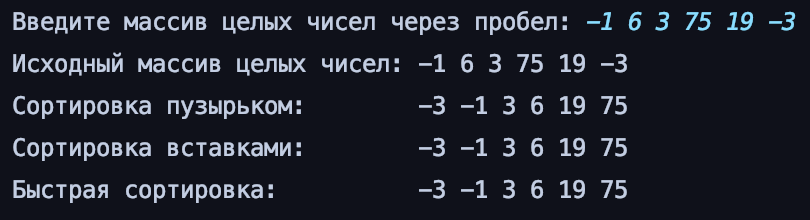
\includegraphics[scale=1.1]{demo.jpg}} 
\caption{Пример работы программы}
\label{ris:example}
\end{figure}

\section{Технические характеристики}

Технические характеристики устройства, на котором выполнялось тестирование:

\begin{itemize}
	\item Операционная система: MacOs Big Sur версия 11.0.1;
	\item Оперативная память: 8 GB;
	\item Процессор: Intel(R) Core(TM) i5-8210Y CPU @ 1.60GHz.
\end{itemize}

Тестирование проводилось на ноутбуке при включённом режиме производительности. Во время тестирования ноутбук был нагружен только системными процессами.


\section{Время выполнения алгоритмов}
Произведено измерение времени работы алгоритмов на случайно сгенерированных, отсортированных по возрастанию и убыванию массивах. Для замера времени была использована функция process\_time\_ns.\\

Измерение было произведено 50 раз и результат был усреднён.\\

На рисунках 4.2 - 4.4 приведены графики отображающие время работы алгоритмов в нано секундах от длины массивов для неупорядоченых, отсортированных по возрастанию, отсортированных по убыванию массивов соответственно.


\begin{figure}[h]
	\centering
	\begin{tikzpicture}
		\begin{axis}[
			axis lines = left,
			xlabel = Длина массива,
			ylabel = Время в нано секундах,
			legend pos=north west,
			ymajorgrids=true
			]
			\addplot[color=red, mark=square] table[x index=0, y index=1] {BubbleNotSorted.dat}; 
			\addplot[color=green, mark=square] table[x index=0, y index=1] {InsertNotSorted.dat};
			\addplot[color=blue, mark=square] table[x index=0, y index=1] {QuickNotSorted.dat};
			
			\addlegendentry{Пузырёк}
			\addlegendentry{Вставки}
			\addlegendentry{Быстрая}
		\end{axis}
	\end{tikzpicture}
	\caption{Сравнение времени сортировок неупорядоченных массивов} \label{plot:NotSorted}
\end{figure}


\begin{figure}
	\centering
\begin{tikzpicture}
\begin{axis}[
    	axis lines = left,
    	xlabel = Длина массива,
    	ylabel = Время в нано секундах,
	legend pos=north west,
	ymajorgrids=true
]
\addplot[color=red, mark=square] table[x index=0, y index=1] {BubbleSortedUp.dat}; 
\addplot[color=green, mark=square] table[x index=0, y index=1] {InsertSortedUp.dat};
\addplot[color=blue, mark=square] table[x index=0, y index=1] {QuickSortedUp.dat};

\addlegendentry{Пузырёк}
\addlegendentry{Вставки}
\addlegendentry{Быстрая}
\end{axis}
\end{tikzpicture}
\caption{Сравнение времени сортировок отсортированных по возрастанию массивов} 
\label{plot:SortedUp}
\end{figure}


\begin{figure}
    \centering
\begin{tikzpicture}
\begin{axis}[
    	axis lines = left,
    	xlabel = Длина массива,
    	ylabel = Время в нано секундах,
	legend pos=north west,
	ymajorgrids=true
]
\addplot[color=red, mark=square] table[x index=0, y index=1] {BubbleSortedDown.dat}; 
\addplot[color=green, mark=square] table[x index=0, y index=1] {InsertSortedDown.dat};
\addplot[color=blue, mark=square] table[x index=0, y index=1] {QuickSortedDown.dat};

\addlegendentry{Пузырёк}
\addlegendentry{Вставки}
\addlegendentry{Быстрая}
\end{axis}
\end{tikzpicture}
\caption{Сравнение времени сортировок отсортированных по убыванию массивов} 
\label{plot:SortedDown}
\end{figure}

\newpage
\section{Вывод}
Были протестированы алгоритмы сортировки на массивах размерами 100…1000 с шагом 100. Рассмотрены нупорядоченные, отсортированные по возрастанию, отсортированные по убыванию массивы.

Экспериментально было подтверждено, что при сортировке отсортированных по возрастанию массивов сортировка вставками показывает наилучший результат.

Исходя из графиков наглядно видно, что сортировка пузырьком является самой медленной.

\chapter*{Заключение}
\addcontentsline{toc}{chapter}{Заключение}
В ходе выполнения данной лабораторной работы были реализованы три алгоритма сортировки: сортировка пузырьком, сортировка вставками и быстрая сортировка. Был проведён анализ каждого алгоритма и измерено время работы алгоритмов для массивов разных размеров. Была оценена трудоёмкость алгоритмов.


\chapter*{Список литературы}
\addcontentsline{toc}{chapter}{Список литературы}
\begin{enumerate}
    \item  Кормен, Т., Лейзерсон, Ч., Ривест, Р., Штайн, К. Глава 7. Быстрая сортировка // Алгоритмы: построение и анализ = Introduction to Algorithms / Под ред. И. В. Красикова. — 2-е изд. — М.: Вильямс, 2005.
    \item Левитин А. В. Глава 4. Метод декомпозиции: Быстрая сортировка // Алгоритмы. Введение в разработку и анализ — М.: Вильямс, 2006. 
\end{enumerate}

\end{document}

